%
% File acl2020.tex
%
%% Based on the style files for ACL 2020, which were
%% Based on the style files for ACL 2018, NAACL 2018/19, which were
%% Based on the style files for ACL-2015, with some improvements
%%  taken from the NAACL-2016 style
%% Based on the style files for ACL-2014, which were, in turn,
%% based on ACL-2013, ACL-2012, ACL-2011, ACL-2010, ACL-IJCNLP-2009,
%% EACL-2009, IJCNLP-2008...
%% Based on the style files for EACL 2006 by 
%%e.agirre@ehu.es or Sergi.Balari@uab.es
%% and that of ACL 08 by Joakim Nivre and Noah Smith

\documentclass[11pt,a4paper]{article}
\usepackage[hyperref]{acl2020}
\usepackage{booktabs}
\usepackage{graphicx}
\usepackage{times}
\usepackage{latexsym}
\renewcommand{\UrlFont}{\ttfamily\small}

\usepackage{microtype}

\aclfinalcopy % Uncomment this line for the final submission


\newcommand\BibTeX{B\textsc{ib}\TeX}

\title{Project Milestone Report\\
{\large Sentiment Analysis on IMDB Movie Reviews Proposal: Developing a Model for Sentiment Classification}}


\author{Lei Yang \\
  Tulane University \\
  {lyang20@tulane.edu} \\\And
  Qinzheng Xu \\
  Tulane University \\
  {qxu5@tulane.edu} \\}

\date{}


\begin{document}
\maketitle
% \begin{abstract}
% Lorem ipsum dolor sit amet, consectetur adipiscing elit, sed do eiusmod tempor incididunt ut labore et dolore magna aliqua. Ut enim ad minim veniam, quis nostrud exercitation ullamco laboris nisi ut aliquip ex ea commodo consequat. Duis aute irure dolor in reprehenderit in voluptate velit esse cillum dolore eu fugiat nulla pariatur. Excepteur sint occaecat cupidatat non proident, sunt in culpa qui officia deserunt mollit anim id est laborum.
% \end{abstract}


\section{Problem Overview}

The issue at hand is using deep learning models to automatically figure out how people feel about movies in reviews. The goal is to correctly find, separate, and label the feelings behind movie reviews from the IMDB database as either positive, negative, or neutral. The subjective and often complicated nature of human language, which includes sarcasm, idiomatic expressions, and different emotional states, makes this job hard. To make things even more difficult, you have to understand the context and semantics of the texts in order to accurately classify the mood. The end goal is to use the information gathered from this research to help entertainment companies improve their services, make their marketing more effective, and make viewers happier. Achieving high accuracy in sentiment analysis can make these insights more open to everyone, so more people can understand and use the feelings and opinions shared in movie reviews.



\section{Data}

This sentiment study is based on information from the IMDB database, which has 50,000 movie reviews. This dataset was carefully chosen for tasks that involve natural language processing and text analytics. Its main focus is on binary mood classification, which means putting reviews into two groups: positive and negative. The data has a lot of it, which makes it a great resource for training and testing deep learning models that are meant to analyse mood. This dataset is unique because it is so big. Compared to other standard datasets in the same field, it lets you train and test models in more ways.

There are two parts to the dataset: a training set and a testing set. Each has 25,000 movie reviews. This fair split makes sure that both positive and negative feelings are represented equally, which is important for teaching computers to correctly sort feelings without any bias. The data comes from the IMDB library and can be found on Kaggle~\citep{maas2011learning}, a website for data science and machine learning projects. In the fields of mood analysis and natural language processing, this makes it easier to repeat studies and make sure that results are correct.





\section{Method}

\subsection{Algorithms Used}

We used three different types of neural networks to figure out how people felt about IMDB movie reviews: Artificial Neural Networks (ANN), Recurrent Neural Networks (RNN), and Transformer models. Each of these models takes a different approach to dealing with and making sense of the complex structure of textual data, and each has its own benefits when it comes to catching the subtleties of language and emotion.

% \begin{itemize}
%     \item \textbf{ANN Model}: As a starting point, the ANN model is used to simulate a sped-up version of the neural processes seen in the human brain. It works by learning patterns and connections in the data through layers of neurones. We used a structure with thick layers and dropout layers in between to keep the model from overfitting and make sure it works well with data it hasn't seen before.
%     \item \textbf{RNN Model}: Textual data is usually stored in a certain order, so the RNN model takes that into account when it comes to processing inputs. The RNN can remember long-term relationships thanks to its Long Short-Term Memory (LSTM) units. This makes it perfect for sentiment analysis, where the order and context of words have a big effect on their meaning.
%     \item \textbf{Transformer Model}: The Transformer architecture introduces an attention mechanism, allowing the model to focus on different parts of the input sequence when making predictions. This approach is highly effective for understanding context and relationships within the text, offering advantages in processing the complex structure of movie reviews.
% \end{itemize}

\subsection{Libraries and Variations}

We used well-known Python tools for deep learning, like TensorFlow and Keras, to put these models into action. These libraries make the development process faster by giving you a lot of tools and features for creating and training neural network models.

\begin{itemize}
    \item We used normal configurations from the Keras library for the ANN and RNN models, but changed the number of units, dropout rates, and sequence processing to make them work best for sentiment analysis.
    \item Because TensorFlow is so flexible, the Transformer model implementation added custom layers and attention mechanisms to make it work for our text classification job.
\end{itemize}

\subsection{Evaluation Methods}

A confusion matrix, which is a powerful way to see how well a model can classify things into different groups, was used to judge the models' success. Accuracy, precision, recall, and the F1 score are some of the key measures we got from the confusion matrix. These metrics give a full picture of how well the model can predict the future and tell the difference between happy and negative emotions.

% \begin{itemize}
%     \item \textbf{Accuracy} measures the overall effectiveness of the model in correctly identifying sentiments.
%     \item \textbf{Precision} and \textbf{Recall} offer insights into the model's ability to correctly predict positive sentiments and minimize false positives.
%     \item \textbf{F1 Score} serves as a balance between precision and recall, providing a single metric to assess the model's overall performance in handling both aspects.
% \end{itemize}

\subsection{Baselines for Comparison}
A comparison with well-known benchmarks in sentiment analysis was part of our research to make sure that our models worked. By comparing our results to these standards, we wanted to show how our method led to progress and possible improvements. We specifically looked at standard metrics that regular machine learning methods and past neural network models got right in sentiment analysis tasks. We then used these as a starting point to see how much better our ANN, RNN, and Transformer models were.


\section{Intermediate/Preliminary Experiment Results}

\subsection{Text Features for Extraction}

We will extract the following text features, each offering unique insights into the text data:

\begin{enumerate}
    \item \textbf{Polarity}: This is a measure ranging from -1.0 to 1.0. A score of 0 denotes neutral sentiment, -1 signifies extremely negative sentiment, and +1 reflects highly positive sentiment.
    \item \textbf{Subjectivity}: Expressed as a float within the range of 0.0 to 1.0. A score of 0.0 indicates a highly objective stance, whereas 1.0 suggests a highly subjective viewpoint.
    \item \textbf{Word Count}: The total number of words present in each review.
    \item \textbf{Part-Of-Speech (POS) Tag Ratios}: We will calculate the ratio of specific POS tags to the total word count in a review. The tags include:
    \begin{itemize}
        \item PROPN (Proper Noun), e.g., John, London, NATO.
        \item PUNCT (Punctuation), e.g., ., (, ), ?, !.
        \item NOUN, e.g., woman, tree, beauty.
        \item ADJ (Adjective), e.g., big, yellow, sparkling.
        \item VERB, e.g., eat, running.
    \end{itemize}
    \item \textbf{Uppercase Ratio}: The proportion of uppercase words to the total word count in the review.
    \item \textbf{Digits Ratio}: The proportion of digits to the total word count in the review.
\end{enumerate}

\subsubsection{Polarity Distribution}
The histogram shows the orientation scores of reviews that are both positive and negative. When reviews are good, the polarity scores are more concentrated on the right side of the scale, reaching their highest point in the range that shows strong positive sentiment. On the other hand, bad reviews have a polarity distribution that leans to the left and has a peak in the negative spectrum. 
\begin{figure}[ht]
    \centering
    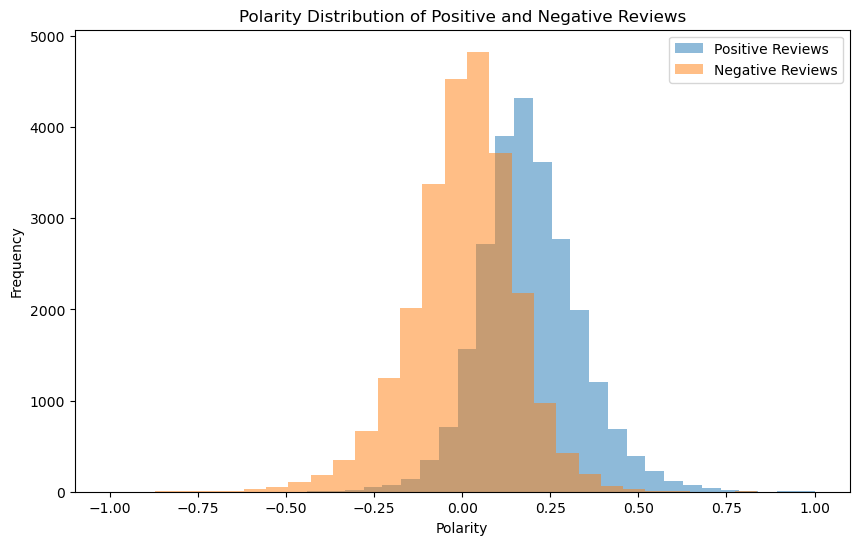
\includegraphics[width=0.5\textwidth]{1.png}
    \caption{Polarity Distribution}
    \label{fig:polarity_distribution}
\end{figure}


This bimodal distribution highlights the clear demarcation between the sentiments of positive and negative reviews, essential for refining sentiment analysis algorithms.

\subsubsection{Word Count Distribution Analysis}
The histogram and boxplot visualization indicate the frequency of word counts for both positive and
\begin{figure}[ht]
    \centering
    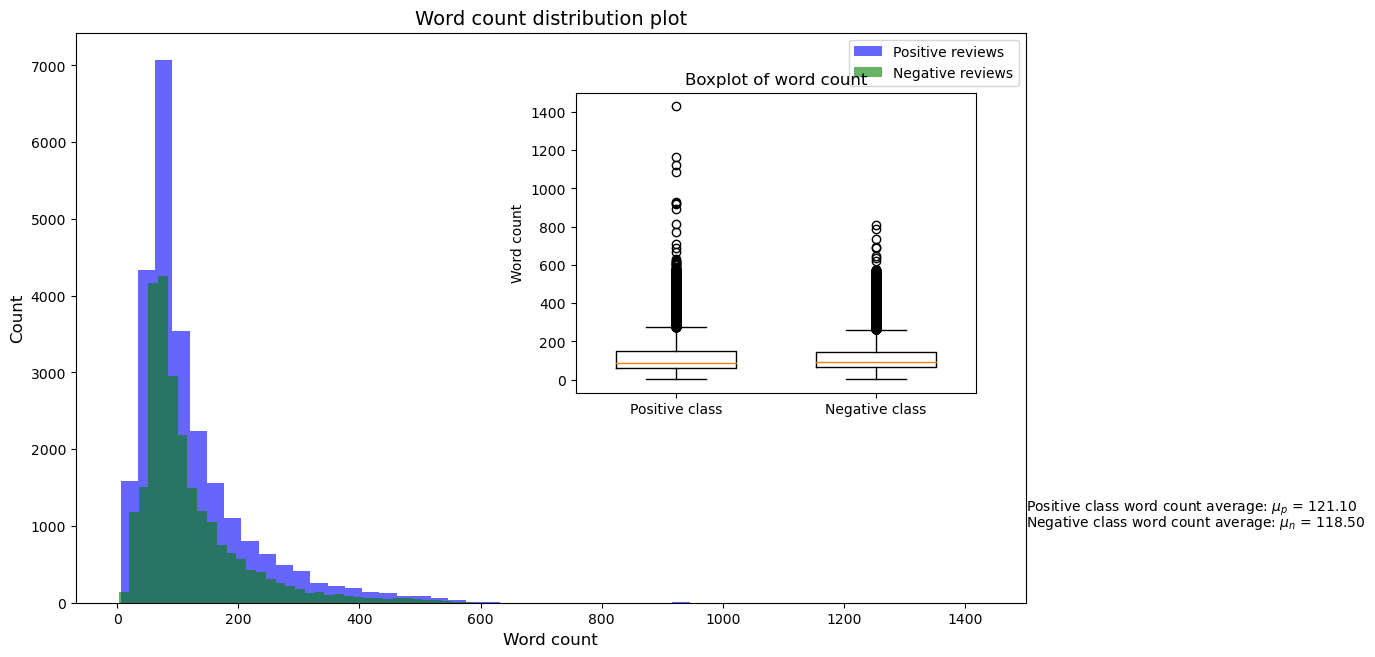
\includegraphics[width=0.5\textwidth]{2.png}
    \caption{Polarity Distribution}
    \label{fig:polarity_distribution}
\end{figure}


\section{Related Work}

When researchers use sentiment dictionaries to study sentiment analysis, the first thing they need to do is label the expression trend of sentiments. This means that they need to make the emotional meanings of words clearer. The study is based on predefined semantic rules and the sentiment scoring of the lexical expressions in the sentiment dictionary. A series of text processing is used to get the general sentiment tendency of the text. Some researchers, including Tureny et al.~\citep{turney2007anatomy}, look at and figure out how similar words are by adding mutual information intent. They also rebuild the dictionary by adding polar semantics, which makes the dictionary's lexical construction more complex. Yang et al.~\citep{chen2013emotional} start with a sentiment dictionary that already exists and use the LDA model tool to find the topic words in that dictionary. This makes the sentiment tendencies more expressive and gives topic words with multiple meanings a lot of extra information. Pang et al.~\citep{pang2002thumbs} were the first to use machine learning to solve the sentiment analysis binary classification problem. They combined standard bag-of-words methods with machine learning to make the classification work better. Wikarsa et al.~\citep{wikarsa2015text} gathered a huge number of Twitter comments as a dataset and then put emotions into groups based on their meanings. Once the groups were made, the authors used standard machine learning algorithms to figure out how people felt about the tweets, taking into account the emojis and words in the dataset to improve the algorithm's performance and accuracy. Govindarajan et al.~\citep{govindarajan2013sentiment} made a big step forward in combining genetic algorithms and traditional machine learning algorithms in a natural way. They used the combined algorithm as a new way to solve the problem of sentiment binary classification and got better results in binary classification effects. Chikersal et al.~\citep{chikersal2015sentu} changed the emotional rules of emojis and polysemous words in comment texts by mixing rule processing and SVM and processing Twitter corpora. This made text semantic prediction more accurate. But the text opinion research based on machine learning has hit a wall. This is because the research field is getting too big. When it comes to current long text jobs that involve semantics, the combination of dictionary rules and machine learning often doesn't work as planned, which slows down research and development.



\section{Division of Labor and Timeline}

\subsection{Division of Labor}

The project tasks have been divided into two main categories: the coding part and the report part. 

\begin{itemize}
    \item \textbf{Coding Part:}
    \begin{itemize}
        \item \textbf{[name1]} will focus on developing the backend algorithms for sentiment analysis, including the implementation of the neural network models and data preprocessing.
        \item \textbf{[name2]} is responsible for the frontend development, creating the user interface for the web application and integrating the backend algorithms.
    \end{itemize}
    
    \item \textbf{Report Part:}
    \begin{itemize}
        \item \textbf{[Qinzheng Xu]} will contribute to writing the methodology section of the report, detailing the algorithms used and the rationale behind model choices.
        \item \textbf{[Lei Yang]} will handle the results and discussion sections, analyzing the performance of the implemented models and discussing the implications of the findings.
    \end{itemize}
\end{itemize}

\subsection{Timeline}

\begin{enumerate}
    \item \textbf{Frontend Development and Integration:} Completion by [March 02, 2024].
    \begin{itemize}
        \item Task involves developing the web application frontend and integrating it with the backend algorithms.
    \end{itemize}
    
    \item \textbf{Testing and Refinement:} Completion by [March 09, 2024].
    \begin{itemize}
        \item This phase focuses on testing the complete system, refining the models based on performance, and ensuring usability of the web interface.
    \end{itemize}
    
    \item \textbf{Final Report Writing:} Completion by [March 15, 2024].
    \begin{itemize}
        \item The final step includes compiling the project report, incorporating all sections, and reviewing the document for completeness and accuracy.
    \end{itemize}
\end{enumerate}






\bibliography{references}
\bibliographystyle{acl_natbib}


\end{document}
